\documentclass{article}    
\usepackage[left=2cm, right=2cm, top=2cm, bottom= 2cm]{geometry} 
\usepackage{hyperref}
\usepackage{graphicx,epsfig,verbatim,enumerate}
\usepackage{amssymb,amsmath,amsthm,amsbsy}
\usepackage{ifthen}
\usepackage{morefloats}
\hypersetup{colorlinks=true, linkcolor=blue}
\usepackage{cite}
\usepackage{color}
\usepackage{textcomp}
\newcommand{\todo}[1]{\noindent\textcolor{blue}{{$\Box$ #1}}}

\title{Project Proposal}
\date{\today}
\author{Luke Trinity and Nat Shenton \\  CS 254}

\begin{document} 
\maketitle
\section{Introduction}

Online sources of high resolution images including Google, Image-net \cite{deng2009imagenet}, and Flickr are providing new opportunities to explore applications of image categorization using computer vision. One interesting application in the field of fine-grained image classification is identification of dog breed. Dogs faces are considered to be highly differentiable for each breed, which makes classification an approachable problem.  However, the work is challenging due to the varying combinations of facial characteristics and color patterns between species, as well as intra-class variation within a single species. Another aspect of the problem that makes it more complicated is the presence of humans and man-made backgrounds, which are not as common in other animal datasets. In addition, many attempts to classify dog breeds fail to corroborate the results with actual DNA evidence. Our approach will be to utilize an existing dog breed image classification dataset \cite{khosla2011novel}, in combination with a novel dataset that includes paired DNA test results and photos \cite{voith2009comparison}, to  classify non-pure bred dog breeds. 

\section{Problem Definition and Algorithm}

\subsection{Task Definition}

The task is to take dog images where each image is labeled with a breed and classify what breed the dog could possibly be.  This will is to normalize these images as the inputs.  Each input image is defined as a matrix of $250\times 250 \times 3$.  The output will the probability that the dog is a certain breed.  This is an interesting problem as it could provide dog owners an easy way to classify a dog breed.  With innovations such as Googles Opensource API which allows for object detection.  Allowing dog owners the ability to classify their pet in terms of the percentages of possible breeds would be a useful tool for dog owners.  The final input for this task would allow for a dog owner to upload a picture of their dog to a website or app and then the machine learning algorithm will classify their dog as a percentage of each breed.  The final output of be the probability of the most likely breeds.

\subsection{Dataset}

The Stanford Dogs Dataset has 20,580 images each classified into one of 120 classes of dog breed. \cite{khosla2011novel} Each image also has an associated bounding box identifying the location of the dog within the photo. The mixed-breed DNA identified dog photo dataset from Voith et al. \cite{voith2009comparison} has 20 images, each paired with DNA percentage breakdown of dog breed. There are no associated bounding boxes for the Voith dataset \cite{voith2009comparison}. We will need to outfit this second dataset with bounding boxes to improve the accuracy of our classification algorithm, when the second phase of the project is reached. Later in the semester we hope to have other mixed breed training data, our backup plan is to scrape dog show images hosted online to generate our own dataset. 

\subsection{Algorithm Definition}
First we will convert each of the images in the Stanford Dogs dataset \cite{khosla2011novel} into a single feature vector based on the trimmed height and width of the images and the (r,g,b) values in each cell. We will then pair the images with their associated class labels, and utilize a neural network as a black box to train our model to accurately predict the class of our test images. Later in the semester we hope to unbox the neural network with more advanced knowledge to achieve better accuracy. One method we will work to implement, which was utilized by both Kohsla et al. \cite{khosla2011novel} and Liu et al. \cite{liu2012dog}, is scale-invariant feature transform (SIFT). This algorithm detects and describes local features in images by finding candidate matching features based on Euclidean distance of feature vectors.  \cite{lowe2004distinctive} After achieving a high level of accuracy classifying pure-bred dogs, we will introduce our other dataset \cite{voith2009comparison} that carries interesting practical concerns in our implementation of SIFT. Here we will attempt to classify mixed breed dogs using images annotated with precise DNA testing of breed composition. Hopefully we can augment this dataset with more samples by reaching out to different labs. This is an interesting computer vision problem because dogs often share features, whether it be color patterns or facial structure, that lead to breed misrepresentation.  Training an algorithm in this capacity could lead to novel conclusions related to classifying a dog as purebred or a mixed breed. 
 
\section{Experimental Evaluation}
\subsection{Methodology}

\subsection{Results}
 \begin{figure}[h!]
 \centering
  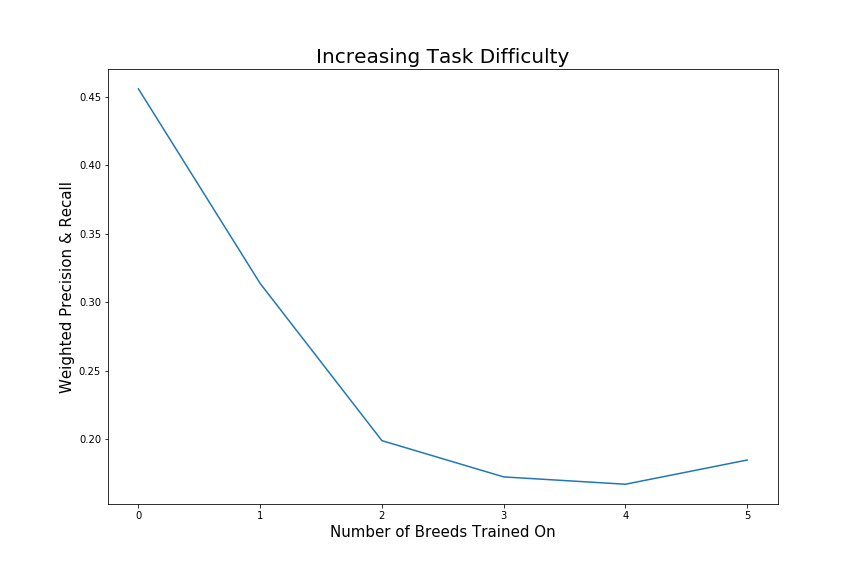
\includegraphics[width=0.7\textwidth]{results}
  \caption{The wieght precision and recall the classification from Keras model}
  \end{figure}
\subsection{Discussion}

 
\section{Related Work}

In the initial article utilizing the novel dataset by Khosla et al. \cite{khosla2011novel}, the mean accuracy reached 22\% when 100 training images were utilized within the SIFT methodology. Liu et al. \cite{liu2012dog} reached 69\% accuracy, with greater success than Khosla et al. \cite{khosla2011novel} due to their partially localized approach.  We hope to leverage the bounding boxes and augment the work of Liu et al. \cite{liu2012dog}, possibly improving on their methodology to achieve higher accuracy. Several bounding box approaches are currently being reviewed, although all are endlessly modifiable from simple image segmentation. One is a slight adaptation to a method often employed for training algorithms to images of different shade and dimension called DeepCut.  \cite{rajchl2016deepcut} There are several standard variations on the basic DeepCut methodology, which hones in on the nature and dimension of the bounding in a cookie-cutter, traced-out way as opposed to any kind of geometric shape. A very similar methodology is known as GrabCut which does not need to even be a single, continuous cookie-cutter-style line bounded around a desired segment of an image. GrabCut is standardly designed to grab multiple disparate segments of an image at once for a single, desired analysis. In addition to one of these approaches or some modification thereof, we plan to incorporate some aspect of KL Loss to account for localization uncertainty which could greatly assist with interference from background objects such as people, buildings, trees, etc. \cite{he2019bounding} There are, of course, a number of other modifiable ‘standard’ or ‘familiar’ combinations of approaches to deal with bounding and uncertainty to also be explored. Even so, most will lead to an approximately similar result if implemented correctly. Deep/GrabCut is simple and can narrow the selected image segment in a convenient, efficient manner. KL Loss will be further researched and incorporated to deal with expected shading difficulties, image blurring and background/foreground image ‘noise’.

\section{Next Steps}

These initial results show the next steps, one is to improve the learning algorithm.  The initial Keras Neural network shows the classification of dog breeds get worse and worse as the more breeds get introduced.  From here, the main goal is to improve this algorithm.  This will be done thru cross-validation and using the Keras pre trained Neural Networks.  These networks 

\todo{use cv to get hyperparameters}\\
\todo{work on memory issue possibly the vacc}

\section{Code and Dataset}

The code can be found in our github repo: \url{https://github.com/nshenton/CS_251_DogProject}.  Please see the Readme in the repo for more information.  The Stanford Dogs Dataset can be downloaded from this page: \url{http://vision.stanford.edu/aditya86/ImageNetDogs/}.

\section{Conclusion}

\bibliography{dogbib}{}
\bibliographystyle{ieeetr}

\end{document}    